\documentclass{article}
\usepackage{graphicx}
\usepackage{listings}
\usepackage{color}
\usepackage{amsmath}
\usepackage{amsfonts}
\usepackage{bm}
\usepackage[utf8]{inputenc}

\title{Modelli di crescita della popolazione\\
	Corso di LSMC, a.a. 2017-2018}
\author{Davide Gori\\
	550282}


\definecolor{backcolour}{rgb}{0.95,0.95,0.92}
\definecolor{gray}{rgb}{0.5,0.5,0.5}
\lstset{basicstyle=\ttfamily\small,
	columns=fullflexible,
	numbers=left,
	numberstyle=\tiny\ttfamily\color{gray},
	backgroundcolor=\color{backcolour},
	tabsize=4,
	language=Octave
}


\begin{document}
	\maketitle
	\section{Prima sperimentazione: colonia di batteri}
	Considero una colonia di batteri. Assumiamo che la sua crescita, determinata da divisioni di cellule, sia caratterizzata dalle seguenti tre proprietà:
	\begin{itemize}
		\item all’inizio la colonia è composta da 1000 batteri.
		\item dopo un’ora il numero di batteri è raddoppiato.
		\item in intervalli temporali di uguale lunghezza il numero di batteri aumenta di uguale fattore.
	\end{itemize}
	Determino il valore dei parametri del modello che descrive questa situazione. \\
	Utilizzando il metodo di Eulero, troverò la soluzione numerica del modello ottenuto e disegnerò il numero di batteri presenti nella colonia nelle prime sei ore.
	
	\subsection{L'implementazione}
	Essendo la velocità di accrescimento costante (per la terza ipotesi) allora abbiamo che y'/y=a costante, sapendo che la soluzione è del tipo $c e^{at}$ sappiamo che, visto che in 1 ora si ha un raddoppiamento della popolazione, $e^a=2$, da cui $a=\ln(2)$.\\
	Siccome f(0)=1000 allora c=1000. Risolviamo ora utilizzando un metodo numerico.
	\subsection{Il codice}
	Questo è lo script che realizza la sperimentazione (viene usato {\tt eulero}, già implementato nelle precedenti esercitazioni):
	\lstinputlisting{LabSper_3_1.m}
	\subsection{Risultati}
	Riportiamo il grafico in output.
	\begin{figure}[htp!]
		\centering 
		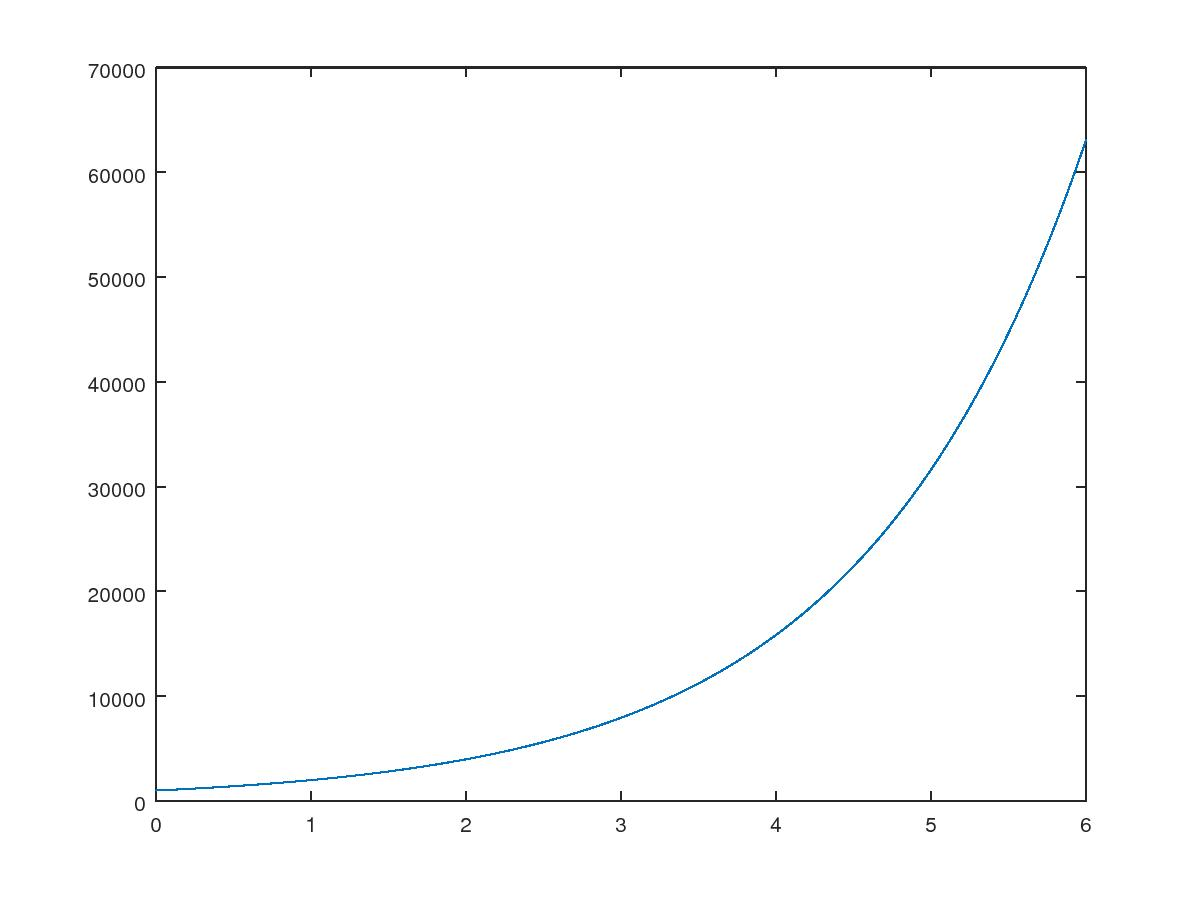
\includegraphics[width=\textwidth]{3_1.jpeg}
	\end{figure}
			\section{Seconda sperimentazione: un esempio}
	La emivita del plutonio è di 50 anni. Troviamo la legge di decadimento e calcoleremo a quanto si riduce un grammo di plutonio dopo 100 anni.\\
	Utilizzando il metodo di Runge-Kutta classico, determino la soluzione numerica del modello ottenuto. Deducendo quanti anni all’incirca occorrono affinché la quantità di plutonio sia $1/10$ di quella iniziale. Rappresentare in un grafico l’andamento della quantità di plutonio presente nei primi 50 anni.
	
	\subsection{L'implementazione}
	Sapendo che la leggi per il decadimento è esponenziale, abbiamo che $y=c e^{at}$ abbiamo che $0.5=\frac{y(t+50)}{y(t)} e^{50a}$.\\
	Dunque $a=-ln(2)/50$. Se dopo 50 anni la quantità è dimezzata, dopo 100 è 1/4 di grammo. Il modello ottenuto risolve la seguente equazione differenziale: $y'=-\frac{\ln(2)}{50} y$, con $y(0)=1$.
	\subsection{Il codice}
	Questo è lo script che realizza la sperimentazione (viene usato {\tt RK4}, già implementato nelle precedenti esercitazioni):
	\lstinputlisting{LabSper_3_2.m}
	\subsection{Risultati}
	Il tempo necessario per decimare la quantità di atomi è $t=-\frac{\ln(10)}{a}=166.10$.
	Riportiamo il grafico in output.
	\begin{figure}[htp!]
		\centering 
		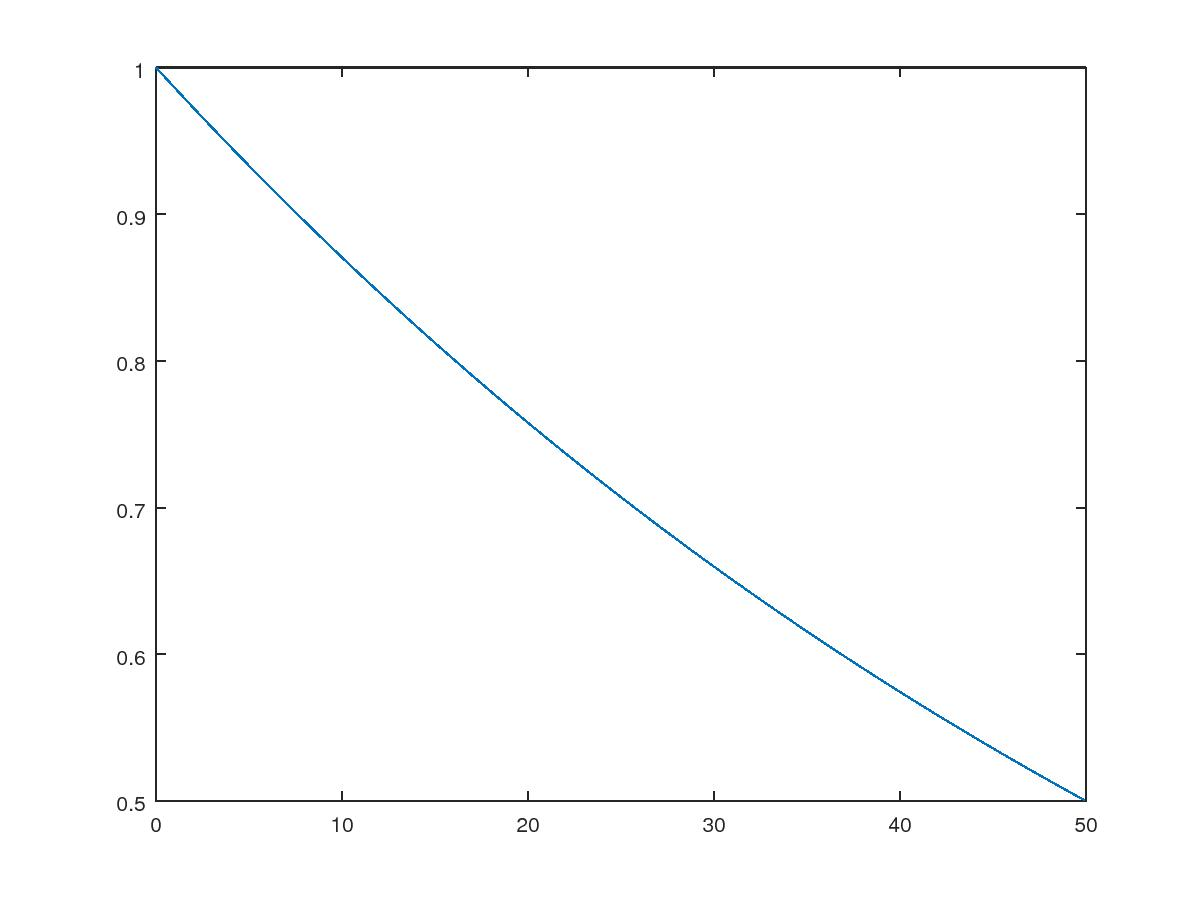
\includegraphics[width=\textwidth]{3_2.jpeg}
	\end{figure}
	
	\section{Terza sperimentazione: un altro esempio}
	Consideriamo una popolazione la cui evoluzione è descritta dall’equazione logistica. Si supponga che la densità iniziale di popolazione sia pari a 2 e che la capacità portante
	dell’ambiente sia $0.01$, con potenziale biologico della popolazione pari a $0.2$. Risolveremo numericamente l’equazione logistica mediante la routine ode45 sull’intervallo $\left[0, 0.5\right]$ e tracceremo il grafico della soluzione stabilendo graficamente a quale istante la densità di popolazione sarà un decimo di quella iniziale.

	\subsection{L'implementazione}
	L'equazione logistica è del tipo $y'=y(a-by)$ dove:
	\begin{itemize}
		\item Capacità portante dell'ambiente: $K=a/b=0.01$.
		\item Potenziale biologico: $a=0.2$.
		\item $y0=2$
	\end{itemize} 
	quindi $b=20$, $a=0.2$ (con riferimento al codice scritto).
	
	\subsection{Il codice}
	Questo è lo script che realizza la sperimentazione:
	\lstinputlisting{LabSper_3_3.m}
	\subsection{Risultati}
	Riportiamo il grafico in output, dal quale si può evincere la soluzione grafica.
	\begin{figure}[htp!]
		\centering 
		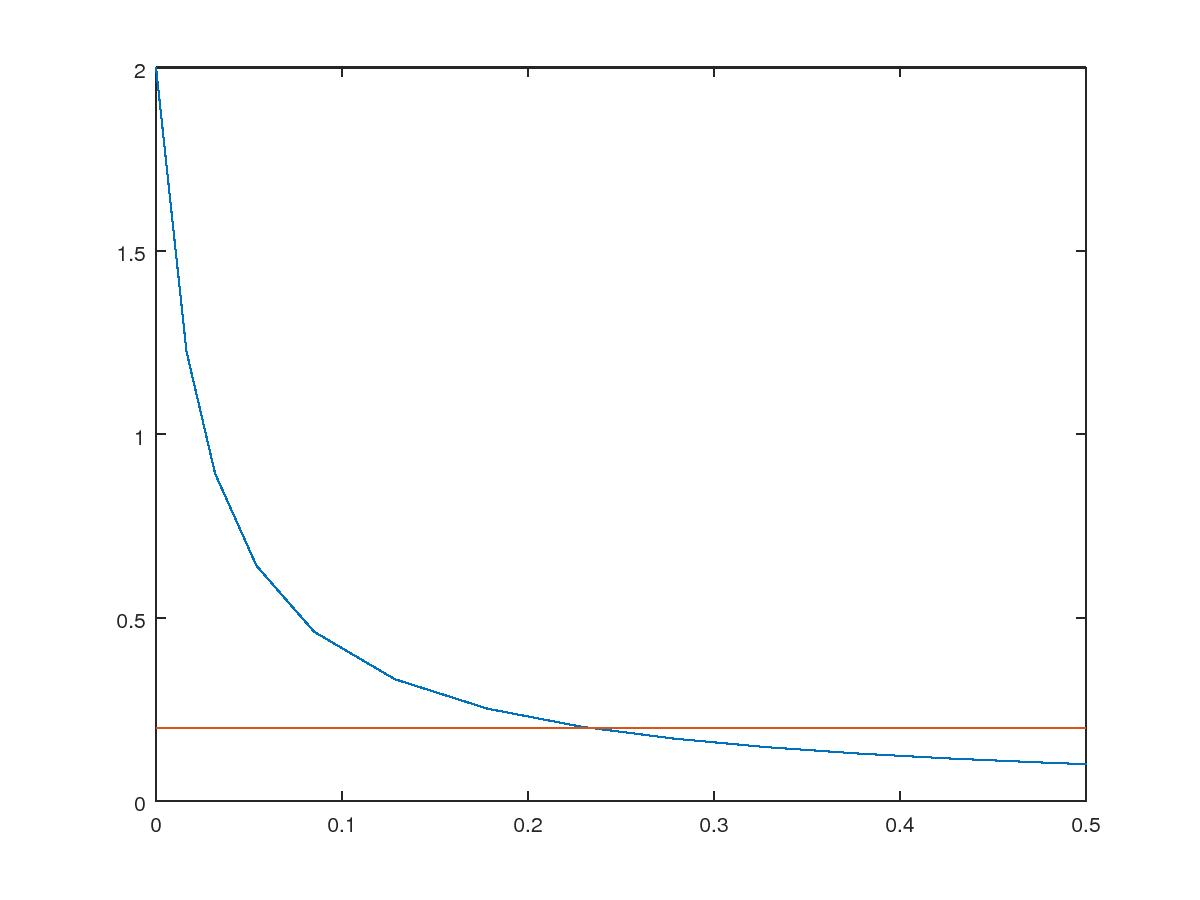
\includegraphics[width=\textwidth]{3_3.jpeg}
	\end{figure}
	\newpage
	\section{Quarta sperimentazione: uno studio}
	Risolverò numericamente l’equazione logistica
		\begin{equation}
	\begin{cases}
	y'=\alpha \left(1-\frac{y}{K}\right) y \\
	y(0)=y_0
	\end{cases}
	\end{equation}
	con il parametro malthusiano dipendente dal tempo nel modo seguente (periodicità stagionale):
	$$\alpha(t)=\frac{1}{2}+ \cos(2 \pi t)$$
	e la capacità portante $K = 100$. Studiare la soluzione in funzione del tempo t.\\
	Disegnerò poi sull’intervallo $\left[0, 20\right]$ il grafico di $y(t)$ per i valori iniziali $y0 = 1, 10, 50, 200$.
	
	\subsection{L'implementazione}
	L'equazione logistica è del tipo $y'=\alpha(t) \cdot y(t) \cdot \left(1-\frac{y}{K}\right)$; dove:\\
	\begin{itemize}
		\item $\alpha(t)=\frac{1}{2}+\cos(2 \pi t)$.
		\item $K=100$.
		\item $y_0=2$.
	\end{itemize}
	quindi $b=20$, $a=0.2$.
	\subsection{Il codice}
	Questo è lo script che realizza la sperimentazione:
	\lstinputlisting{LabSper_3_4.m}
	\subsection{Risultati}
	Possiamo notare che se $y_0>K$ abbiamo una soluzione decrescente, negli altri casi cresce. In generale la soluzione è simile a quella del caso classico in cui $\alpha$ è costante.\\
	Riportiamo il grafico in output.
	\begin{figure}[htp!]
		\centering 
		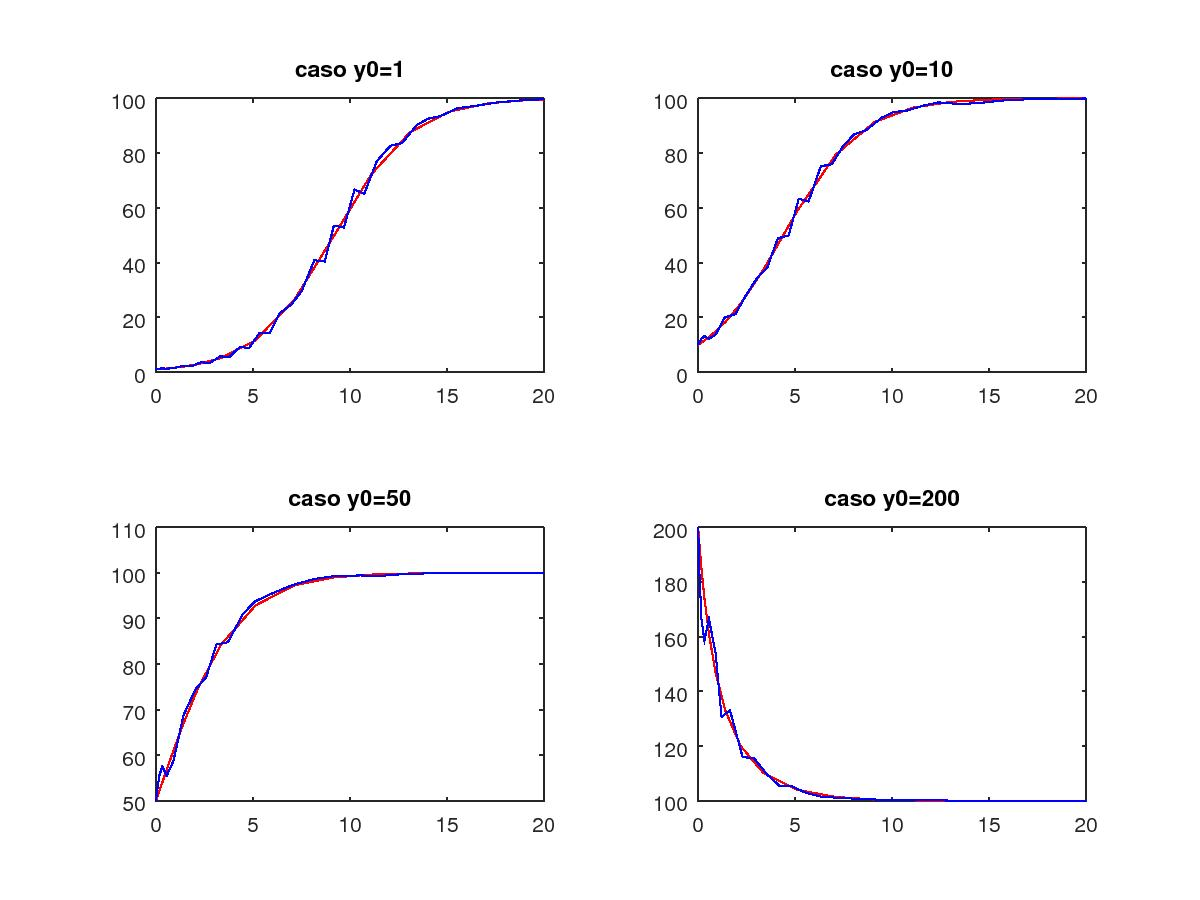
\includegraphics[width=\textwidth]{3_4.jpeg}
	\end{figure}
	
\end{document}